\chapter[cakirxVya saMKeyxgaLu ({\rm\bfseries Cyclic Numbers})]{cakirxVya saMKeyxgaLu\\ ({\rm\bfseries Cyclic Numbers})}
\vskip -20pt

ELu eMba aviBAjayx saMKeyxyiMda oMdanunx BAgisidAga, BAgalabadhxdalilx baruva oMdu guMpu aMkagaLu punarAvatiRsutatxve. ivugaLanunx AvataRka dashamAMsha aMkagaLu enunxtetxVve.
$$
\frac{1}{7} = 0.14285{\dot 7}
$$
ililx eDatudiyalilxruva dashamAMsha biMdu matutx balatudiya koneya aMkada meVliruva AvataRsUcaka biMduvanunx biTuTx biTaTxre $142857$ barutatxde. idoMdu {\bf cakirxVya saMKeyx.} EkeMdare $7$ kikxMta kaDime pUNARMkagaLiMda guNisidare baruva guNalabadhxdalilx saMKeyxgaLu cakirxVyavAgirutatxve.
\vskip 3pt

\begin{minipage}{0.4\textwidth}
\begin{tabular}[c]{>{$}l<{$}}
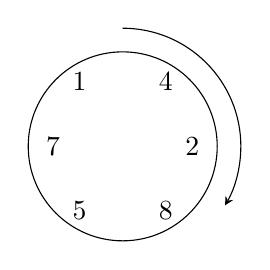
\begin{tikzpicture}[label distance=0.5cm]%%m_073
\draw (1,1) node[circle,
label=60:$4$,label=120:$1$,label=180:$7$, label=240:$5$,
label=300:$8$, label=360:$2$]{}circle(1.2cm);
\draw [>=stealth,->] (1,2.5) arc [radius=1.5, start angle=90, end angle= -30];
\end{tikzpicture}
\end{tabular}
\end{minipage}
\begin{minipage}{0.6\textwidth}
\begin{tabular}[c]{>{$}l<{$}@{\hspace{3pt}}>{$}l<{$}}
142857 \times 1 &= 142857\\
142857 \times 2 &= 285714\\
142857 \times 3 &= 428571\\
142857 \times 4 &= 571428\\
142857 \times 5 &= 714285\\
142857 \times 6 &= 857142
\end{tabular}
\end{minipage}
\vskip 4pt
I saMKeyxgaLalilx $3,6,0$ matutx $9$ elUlx baMdilalx.

$142857$ nunx $7$ riMda guNisidAga $999,999$ barutatxde.

ideV riVti $17$ riMda $1$ nunx BAgisidare
\begin{align*}
\frac{1}{17} &= 0.0588235294117647\\
&\qquad 0588235294117647 \quad\text{oMdu cakirxVya saMKeyx.}
\end{align*}
$588235294117647$ nunx AraMBavAgi $0$ yanunx seVrisabeVku.

$5882352941176470$ oMdariMda hadinArara tanaka saMKeyxgaLiMda guNisidAga guNalabadhx cakirxVyavAgirutatxde.

Adare $17$ riMda guNisidAga $999,999,999,999,999,0$
\begin{align*}
\text{ideV riVti} \;\frac{1}{19} &=  526, 315, 789, 473, 684, 210\\
&\quad ~(18\; \text{ aMkagaLu)  ivU saha cakirxVya saMKeyxgaLu}\\[0.1cm]
\text{ideV riVti}\; \frac{1}{23} &=  0.{\dot 0}43478260869565217391{\dot 3}\; (22 \;\text{aMkagaLu)}\\
\text{ideV riVti} \;\frac{1}{27} &=  0.037 \;(3 \;\text{aMkagaLu)}\\
\text{ideV riVti} \;\frac{1}{29} &=  344,827,586,206,896,551,724,137,931,0\\
&\quad ~(28\; \text{ aMkagaLu)};\\
\text{ideV riVti} \;\frac{1}{31} &=  0.32258064516129\\
&\quad(15\; \text{ aMkagaLu)};\\
\text{ideV riVti}\;\frac{1}{63} &=   0.15873 \text{ivU saha cakirxVya saMKeyxgaLu}\\
 &\quad ~(6\; \text{ aMkagaLu)};
\end{align*}

ideV riVti $1$ nunx $13$ riMda BAgisidAga baruva $076923$ iMdoMdu cakirxVya saMKeyx
$$
\frac{1}{13} = 0.076923
$$
\begin{align*}
076923 \times 1 &= 076923 \\
~~~~~~~~~\shortparallel ~~~\times 3 &= 230769 \\ 
076923\times 4 &= 307692 \\
076923\times 9 &= 692307 \\ 
~~~~~~~~~~~\shortparallel ~\times 10 &= 769230 \\
076923\times 12 &= 923076\\[5pt] 
076923 \times 2 &= 153846 \\
~~~~~~~~~\shortparallel ~~~\times 5 &= 384615 \\
076923   \times 6 &= 461538 \\
~~~~~~~~~\shortparallel ~~~\times 7 &= 538461 \\
~~~~~~~~~\shortparallel ~~~\times 8 &= 615384 \\
~~~~~~~~~~~\shortparallel ~\times 11 &= 846153 
\end{align*}

$076923$ nunx  I eraDu riVtiya saMKeyxgaLiMda guNisidare mAtarx saMKeyxgaLu cakirxVyavAgi barutatxve. modalaneya guMpinalilxruva saMKeyxgaLu eraDaneya guMpinalilxlalx. aMtU saMKeyxgaLa vinAyxsaveV oMdu sobagu! $076923$ nunx $13$ riMda guNisidare $999,999$ barutatxde.
